\newpage
\section{Diagramas de secuencia}
A continuación se describe la interacción de nuestras entidades de negocio y el ciclo de vida que tendrán en la aplicación. También se detalla la interacción,mensajes y la lógica implementada por cada uno de los diferentes escenarios.\par
\subsection{Registro}
El registro de un usuario nuevo consiste en capturar el correo, nombre y una contraseña. Esta captura sera tratada como un JSON el cual viajara atravéz de un método POST. Gateway se encargara de redirigir esta petición al servicio de registro. Este servicio viajara hacia RDS donde se enviara un INSERT para registrar los datos. Si el usuario y la contraseña se encuentra repetido, se enviara un mensaje de error, como se muestra en la figura 3.7
\begin{figure}[h!]
	\centering
	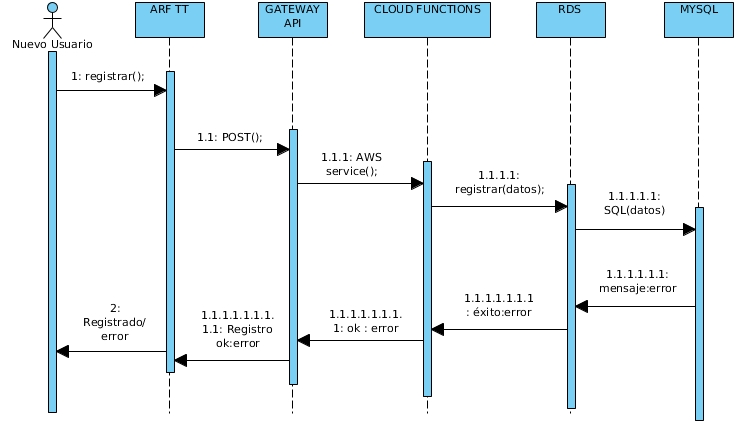
\includegraphics[width=14cm,height=8cm]{imagenes/analisis/DSregistrarUsuario.jpg}
	\caption{Diagrama de secuencia - Registrar usuario.}
	\label{fig:analogo}
\end{figure} 
